%%%%%%%%%%%%%%%%%%%%%%%%%%%%%%%%%%%%%%%%%%%%%%%%
% E.Pinault-Bigeard - s2i@pinault-bigeard.com
% http://s2i.pinault-bigeard.com
% CC BY-NC-SA 2.0 FR - http://creativecommons.org/licenses/by-nc-sa/2.0/fr/
%%%%%%%%%%%%%%%%%%%%%%%%%%%%%%%%%%%%%%%%%%%%%%%%
\documentclass[10pt]{article}

%%%%%%%%%%%%%%%%%%%%%%%%%%%%%%%%%%%%%%%%%%%%%%%%
% Package UPSTI_Document
%%%%%%%%%%%%%%%%%%%%%%%%%%%%%%%%%%%%%%%%%%%%%%%% 
\RequirePackage[QCM,noTypographie]{UPSTI_Document}             
\RequirePackage{multicol}

%---------------------------------%
% Paramètres du package
%---------------------------------%

% Variante
\newcommand{\UPSTIvariante}{2}

% Classe
% 1: PTSI				6: PSI*			11: TSI2		16: Spé
% 2: PT	(par défaut)	7: MPSI			12: ATS
% 3: PT*				8: MP			13: PC
% 4: PCSI				9: MP*			14: PC*
% 5: PSI				10: TSI1		15: Sup
\newcommand{\UPSTIidClasse}{2}

% Type de document
% 1: Cours (par défaut)		8: Fiche Synthèse    		15: Programme de colle 
% 2: TD     				9: Formulaire				16: QCM
% 3: TP						10: Memo
% 4: Colle					11: Dossier Technique
% 5: DS						12: Dossier Ressource
% 6: DM						13: Concours Blanc
% 7: Fiche Méthode			14: Document Réponses
\newcommand{\UPSTIidTypeDocument}{16} % QCM

% Titre dans l'en-tête
\newcommand{\UPSTItitreEnTete}{Théorie des mécanismes - Liaison pivot}      

% Durée de l'activité (pour DS, DM et TP)
\newcommand{\UPSTIduree}{15 min} 

% Numéro (ajoute " n°1" après DS ou DM)
\newcommand{\UPSTInumero}{3}

% Version du document
\newcommand{\UPSTInumeroVersion}{1.0}

%----------------------------------------------- 
\UPSTIcompileVars		% "Compile" les variables
%%%%%%%%%%%%%%%%%%%%%%%%%%%%%%%%%%%%%%%%%%%%%%%% 

%---------------------------------%
% Barême
%---------------------------------%
% Barême pour les questions simples
% 	e = incohérent
% 	v = vide
% 	b = bonne
% 	m = mauvaise
\baremeDefautS{e=0,v=0,b=2,m=-0.5}

% Barême pour les questions multiples
% 	e = incohérent
% 	v = vide
% 	b = bonne
% 	m = mauvaise
% 	formula = Une formule "maison" que j'ai faite. Elle se lit comme ceci : 
\baremeDefautM{e=0,v=0,formula=(NBC+NMC>0 ? -0.25*NMC+1*NBC : ( NB>0 ? 0 : 0 ))}

%%%%%%%%%%%%%%%%%%%%%%%%%%%%%%%%%%%%%%%%%%%%%%%% 
% Début du document
%%%%%%%%%%%%%%%%%%%%%%%%%%%%%%%%%%%%%%%%%%%%%%%% 
\begin{document}


%---------------------------------%
% Groupes de question
%---------------------------------%

\element{tdm}{
%*************************%
\begin{question}{liaisonsParallele}
Pour 2 liaisons en parallèle, que peut-on écrire ?
\begin{reponseshoriz}
	\bonne{$\tAM[eq]{1}{2}[A]=\tAM[A]{1}{2}[A]+\tAM[B]{1}{2}[A]$}
	\mauvaise{$\tAM[eq]{1}{2}[A]=\tAM[A]{1}{2}[A]=\tAM[B]{1}{2}[A]$}
\end{reponseshoriz}
\end{question}

\begin{question}{liaisonsSerie}
Pour 2 liaisons en série, que peut-on écrire ?
\begin{reponseshoriz}
	\bonne{$\tV[eq]{2}{1}[A]=\tV[A]{2}{1}[A]+\tV[B]{2}{1}[A]$}
	\mauvaise{$\tV[eq]{2}{1}[A]=\tV[A]{2}{1}[A]=\tV[B]{2}{1}[A]$}
\end{reponseshoriz}
\end{question}

\begin{question}{nombreCyclomatique}
Que représente le nombre cyclomatique $\nCyclomatique$ ?
\begin{reponses}
	\bonne{Le nombre de boucles cinématiques indépendantes}
	\mauvaise{Le nombre de pièces qu'on peut isoler pour appliquer le PFS}
	\mauvaise{Le nombre de liaisons}
	\mauvaise{Le nombre de pièces}
\end{reponses}
\end{question}
%*************************%
}

\element{tdmExemple}{
%*************************%
\vspace{-1em}
\noindent
\begin{minipage}{\linewidth}
\begin{minipage}[c]{0.46\linewidth}

\begin{question}{Mobilites}
\noindent Soit le micromoteur décrit par le schéma cinématique spatial et le graphe des liaisons ci-contre. Que vaut l'indice de mobilité $m$ ?
\begin{reponseshoriz}
	\bonne{1}
	\mauvaise{0}
	\mauvaise{2}
	\mauvaise{3}
\end{reponseshoriz}
\end{question}

\begin{question}{Ic}
Donner le nombre d'inconnues cinématiques $I_c$.
\begin{reponseshoriz}
	\bonne{6}
	\mauvaise{4}
	\mauvaise{12}
	\mauvaise{18}
\end{reponseshoriz}
\end{question}

\begin{question}{Ec}
Donner le nombre d'équations cinématiques $E_c$.
\begin{reponseshoriz}
	\bonne{6}
	\mauvaise{3}
	\mauvaise{12}
	\mauvaise{18}
\end{reponseshoriz}
\end{question}
\end{minipage}\hfill
\begin{minipage}[c]{.2\linewidth}
	\centering
	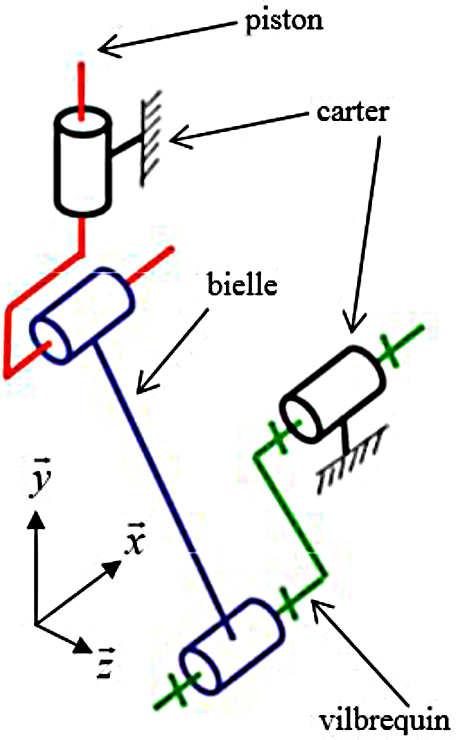
\includegraphics[width=3cm]{Images/sc.png}
\end{minipage}\hfill
\begin{minipage}[c]{0.3\linewidth}
	\centering
	\begin{grapheLiaisons}[scale=0.3]
	\glBati{0,0}{C}{C}[1/0.3]
	\glPiece{-5,5}{V}{V}
	\glPiece{0,10}{B}{B}
	\glPiece{5,5}{P}{P}
	\glLiaison[bend left=20]{C}{V}[Pivot\\ axe \vx{}][left]
	\glLiaison[bend left=20]{V}{B}[Pivot\\ axe \vx{}][left]
	\glLiaison[bend left=20]{B}{P}[Piv. Gl.\\ axe \vx{}][right]
	\glLiaison[bend left=20]{P}{C}[Piv. Gl.\\ axe \vy{}][right]
	\end{grapheLiaisons}
\end{minipage}
\end{minipage}
%*************************%

%*************************%
\begin{question}{h}
Quel est le degré d'hyperstatisme $h$ ?
\begin{reponseshoriz}
	\bonne{1}
	\mauvaise{0}
	\mauvaise{2}
	\mauvaise{3}
	\mauvaise{4}
	\mauvaise{12}
	\mauvaise{-1}
	\mauvaise{$\pi$}
\end{reponseshoriz}
\end{question}
%*************************%

%*************************%
\begin{question}{remplacementLiaison}
Que se passe-t-il si on remplace la liaison \liaison{P}{B} par une linéaire annulaire ?
\begin{multicols}{2}
\begin{reponses}
	\bonne{Le mécanisme devient isostatique}
	\mauvaise{Le mécanisme devient instable}
	\mauvaise{Le mécanisme ne fonctionne plus}
	\mauvaise{Ça ne change rien}
\end{reponses}
\end{multicols}
\end{question}
%*************************%
}

\element{pivot}{
%*************************%
\begin{question}{criterepV}
Quel est le critère principal pour dimensionner un palier lisse
\begin{multicols}{2}
\begin{reponses}
	\bonne{Le produit $pV$}
	\mauvaise{La vitesse $V$}
	\mauvaise{La pression $p$}
	\mauvaise{La qualité $Q$}
\end{reponses}
\end{multicols}
\end{question}
%*************************%

%*************************%
\begin{question}{montagePalierLisse}
Comment doit être monté un palier lisse ?
\begin{multicols}{2}
\begin{reponses}
	\bonne{Serré dans l'alésage}
	\mauvaise{Serré sur l'arbre}
	\mauvaise{Serré sur l'arbre et l'alésage}
	\mauvaise{Glissant sur l'arbre et l'alésage}
\end{reponses}
\end{multicols}
\end{question}
%*************************%

%*************************%
\begin{question}{choixRoulements}
Une liaison pivot par roulements est fortement chargée axialement et radialement. Je vais utiliser:
\begin{multicols}{2}
\begin{reponses}
	\bonne{2 roulements à rouleaux coniques}
	\mauvaise{2 roulements à rouleaux cylindriques}
	\mauvaise{1 roulement à double rangée de billes}
	\mauvaise{1 butée à billes}
\end{reponses}
\end{multicols}
\end{question}
%*************************%

%*************************%
\begin{question}{ajustementRoulement}
Quelle est la bague du roulement qui doit être montée serrée ?
\begin{multicols}{2}
\begin{reponses}
	\bonne{Celle qui tourne par rapport à la charge}
	\mauvaise{Celle qui est fixe par rapport à la charge}
	\mauvaise{Les deux}
	\mauvaise{Aucune des deux}
\end{reponses}
\end{multicols}
\end{question}
%*************************%

%*************************%
\begin{question}{calculDureeDeVie}
Quelle est la formule de la durée de vie pour un roulement rigide à billes ?
\begin{multicols}{2}
\begin{reponses}
	\bonne{$L_{10}=\left(\dfrac{C}{P}\right)^3$}
	\mauvaise{$L_{10}=\left(\dfrac{P}{C}\right)^3$}
	\mauvaise{$L_{10}=\left(\dfrac{C}{P}\right)^{\frac{10}{3}}$}
	\mauvaise{$L_{10}=X.F_r+Y.F_a$}
\end{reponses}
\end{multicols}
\end{question}
%*************************%

%*************************%
\begin{question}{chargeAxialeRoulement}
Pour une liaison à 2 roulements à rouleaux coniques, peut-on déterminer facilement la charge axiale de chacun des roulements ?
\begin{multicols}{2}
\begin{reponses}
	\bonne{Non, il faut d'abord déterminer celui qui fonctionne avec jeu}
	\mauvaise{Non, c'est impossible}
	\mauvaise{Oui, sans problème}
	\mauvaise{Oui, mais il faut changer un des 2 roulements pour rendre le montage isostatique}
\end{reponses}
\end{multicols}
\end{question}
%*************************%


%*************************%
\begin{questionmult}{usureRoulement}
Lesquels de ces éléments ont une influence sur l'usure par fatigue des roulements ?
\begin{multicols}{2}
\begin{reponses}
	\bonne{le nombre de tours}
	\bonne{l'intensité des charges}
	\bonne{la direction des charges}
	\mauvaise{la vitesse de rotation}
	\bonne{la taille des roulements}
	\mauvaise{la taille du carter}
	\mauvaise{le nombre d'arrêts axiaux}
\end{reponses}
\end{multicols}
\end{questionmult}
%*************************%
}

%---------------------------------%
% Début du questionnaire
%---------------------------------%
% Nombre d'exemplaires (c'est plus flexible de définir le nombre d'exemplaire directement dans AMC)
\exemplaire{1}{

% En-tête	
\UPSTIbuildPage
\UPSTIamcZoneIdentification

\vspace{-2.5em}
\section{Théorie des mécanismes}
\cleargroup{tdm}
\melangegroupe{tdm}\copygroup[1]{tdm}{tout}
\restituegroupe{tdm}

\restituegroupe{tdmExemple}

\vspace*{-1em}
\section{Liaison pivot}
\cleargroup{pivot}
\melangegroupe{pivot}\copygroup[1]{pivot}{tout}
\restituegroupe{pivot}
\clearpage    
}
\end{document}
